
\documentclass[11pt,a4paper]{article}
\usepackage[hyperref]{naaclhlt2019}
\usepackage{times}
\usepackage{latexsym}
\usepackage{graphicx}

\usepackage{url}

\aclfinalcopy 

\title{Lyrical Distinction}

\author{Jesse Bartola \\
  {\tt jbartola@} \\\And
  Phil Michalowski \\
  {\tt pmichalowski@ } \\\And
  Nischal Tamang \\
  {\tt ntamang@} \\\And
  Max Berezin \\
  {\tt mberezin@} \\}
  
% \setlength\textwidth{16.0cm}
\date{}

\begin{document}
\maketitle

\section{Introduction}
Music is an important part of our everyday lives. Technological advances in modern society have made it easier than ever for new artists to distribute their songs over the Internet. Unfortunately, the massive volume of songs that are regularly released into the public can make it difficult to discern which song is made by which artist. Moreover, a more important question arises: Are the most popular artists the ones with the most distinct music?

Aside from sound, the words an artist uses in a song are perhaps the most important determining factor in how it will appeal to the public. 
Lyrics contain semantic relevance, which allows for the possibility of implicit analysis of a song's cultural relevance. 
Some of the greatest artists of all time are renown for their unique use of lyricism. Our project will aim to determine if (a) Given a set of lyrics, we can predict with a high degree of certainty who the artist is, and (b) Given our trained prediction model, we can rank artists by their relative lyrical uniqueness and use that to predict their popularity.


\section{Related work}
There exists many research projects on the topic of music genre classification. \newcite{Tsaptsinos} attempts to classify music genres from lyrics using Hierarchical Attention Networks (HAN). 
HAN outperforms N-gram, SVM, KNN and Naive Bayes by utilizing the property that words combine to make lines, lines combine to make segments, and segments combine to make the entire lyrical content.
It recognizes that the semantics of lyrics are embedded in the ordering of content within these levels. 
HAN works by extracting these layers and learning the importance of words, lines and segments. 
To represent the words being fed into the HAN, Tsaptsinos uses 100 dimensional GloVe embeddings. 
GloVe outperforms similar word2vec and SVM based models. 
A benefit of this approach is we do not have to hand pick features.
A negative aspect of this approach is that we do not possess familiarity with the processes, and there would be a learning curve for using both HAN and GloVe. 
This approach performs with an accuracy of 49.50\% whereas a higher value would be ideal. 

In an additional paper, \newcite{FellAnndSporleder} try to classify genre, distinguish quality, and determine the release year of a chosen lyrical passage. 
Unlike Tsaptsinos, Fell \& Sporleder do not use a kind of Neural Network. 
Instead they designed 13 total features including top 100 n-grams, type-token ratio, slang words, part of speech/chunk tags, length of lines, echoisms, rhyme features, imagery, pronouns, past tense, chorus, title and repetitive structures. 
As baseline, they used a simple N-gram model. 
For their main approach they make use of the stylistic features, which are the latter 12 features, along with SVMs. 
Here the thoroughly developed features capture the core aspects of a songs lyrical content. 
The simple methods of N-grams and SVMs had on average 52.5\% accuracy, so this is a process that works quite well. 
However, choosing features might be a tedious task, especially if we want additional features more than ones already used previously. 

\section{Your approach}
How do you plan to solve the problem you chose? Will you approach it differently from previous work or do you plan to try to replicate an existing paper?\footnote{If you choose replication, remember that you have to implement the majority of the code yourself! Do not just copy the authors' Github code, because we will find out.} Remember that this project should take $\sim 2$ months of work!

\paragraph{What baseline algorithms will you use?}
A baseline algorithm is one that is very simple and trivial to implement. For example, “predict the most common class,” or “tag all capitalized words as names,” or “select the first sentence in the document”. Sometimes it can be difficult to get a fancy algorithm to beat a baseline. “Always ask yourself, ‘What’s the simplest experiment I could do to (in)validate my hypothesis?’ Talented researchers have a knack for coming up with simple baselines.”

\subsection{Milestones \& Schedule}
Divide your project into subtasks and estimate how much time each will take. If your group plans to divide subtasks amongst itself, also write who will be responsible for each milestone. If you plan to work on everything together, please say so here. Definitely budget some time for writing the progress report and final report, as well as performing an in-depth analysis of any models you build and/or data you collect. Sample schedule below:
\begin{enumerate}
    \item Acquire and preprocess data (1 week)
    \item Build models for task (3 weeks)
    \item Write progress report! (due Nov. 16)
    \item Analyze the output of the model, do an error analysis (2 weeks)
    \item Work on final report and presentation (2 weeks)
\end{enumerate}

\begin{figure}[t]
    \centering
    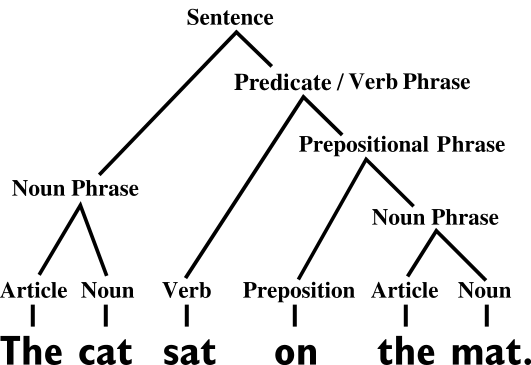
\includegraphics[width=0.5\textwidth]{figs/sentence.png}
    \caption{Please feel free to include figures! If you want your figure to span both columns, use \emph{figure*} instead of \emph{figure}.}
    \label{fig:example}
\end{figure}

\section{Data}
There are many online datasets available containing song lyrics with their respective artists.

What text data do you plan to use in your project? Where will you get it from? Will you be annotating text yourselves? Convince us that it is available for you, and that you can easily get it, and that it is appropriate for the task and research questions you care about.

\section{Tools}
What existing libraries or toolkits are you going to use? 
Some questions to think about: will you be doing any preprocessing of your data such as tokenization or parsing? 
Will you be training logistic regression models? Will you be using deep learning libraries? 
Will you need to use any services for GPUs?\footnote{if so, check out \url{https://colab.research.google.com}!} 
Do you need to use crowdsourcing?

\bibliographystyle{apalike}
\footnotesize
\bibliography{yourbib}


\end{document}
